\documentclass[11pt,a4paper]{article}

\usepackage[utf8]{inputenc}
\usepackage[T1]{fontenc}
\usepackage[brazil]{babel}
\usepackage{lmodern}
\usepackage{amsmath,amssymb,amsfonts,amsthm}
\usepackage{geometry}
\geometry{a4paper, left=20mm, right=20mm, top=22mm, bottom=22mm}
\usepackage{graphicx}
\usepackage{booktabs}
\usepackage{tabularx}
\usepackage{array}
\usepackage{xcolor}
\usepackage{microtype}
\usepackage{hyperref}
\usepackage{fancyhdr}
\usepackage{caption}
\usepackage{float}

\hypersetup{
    colorlinks=true,
    linkcolor=blue!80!black,
    citecolor=blue!80!black,
    urlcolor=blue!80!black,
    pdftitle={Entrega I - Estudo Comparativo Qwen2.5-7B vs Bespoke-Nimble-9B - Mestrado PPGEE/UFAM},
    pdfauthor={Programa de Pós-Graduação em Engenharia Elétrica (PPGEE/UFAM)}
}

\pagestyle{fancy}
\fancyhf{}
\fancyhead[L]{\small\textcolor{gray}{Mestrado PPGEE/UFAM $\bullet$ Entrega I: Análise Comparativa Qwen2.5-7B vs. Bespoke-Nimble-9B}}
\fancyhead[R]{\small\textcolor{gray}{\thepage}}
\fancyfoot[L]{\small\textcolor{gray}{Programa de Pós-Graduação em Engenharia Elétrica -- Universidade Federal do Amazonas}}
\fancyfoot[R]{\small\textcolor{gray}{Novembro de 2026}}
\renewcommand{\headrulewidth}{0.4pt}
\renewcommand{\footrulewidth}{0.4pt}

\theoremstyle{definition}
\newtheorem{definition}{Definição}
\newtheorem{theorem}{Teorema}
\newtheorem{lemma}{Lema}
\newtheorem{corollary}{Corolário}

\definecolor{ufamblue}{RGB}{15, 45, 105}

\begin{document}

\begin{titlepage}
    \centering
    \vspace*{0.4cm}
    {\Huge\bfseries\color{ufamblue} UNIVERSIDADE FEDERAL DO AMAZONAS \par}
    \vspace{0.25cm}
    {\Large\bfseries Faculdade de Tecnologia -- FT \par}
    {\large Programa de Pós-Graduação em Engenharia Elétrica -- PPGEE \par}
    {\normalsize Curso de Mestrado Acadêmico em Engenharia Elétrica \par}
    \vspace{1.0cm}
    
    \rule{\linewidth}{1.5pt} \\[0.4cm]
    {\large\bfseries ENTREGA CIENTÍFICA I \par}
    \vspace{0.25cm}
    {\LARGE\bfseries Estudo Comparativo da Estabilidade Lipschitz e Fidelidade de Quantização na Verificação Formal de Modelos de Linguagem: Qwen2.5-7B versus Bespoke-Nimble-9B \par}
    \rule{\linewidth}{1.5pt} \\[0.9cm]
    
    \begin{minipage}{0.96\textwidth}
        \small
        \begin{tabularx}{\linewidth}{l X}
            \textbf{Programa Acadêmico:} & Mestrado em Engenharia Elétrica (PPGEE -- FT/UFAM) \\
            \textbf{Linha de Pesquisa:} & Controle, Automação, Métodos Formais e Sistemas Inteligentes \\
            \textbf{Padrão Metodológico:} & Estrutura Canônica IMRaD com Rigor Matemático Internacional (\textit{CAV / IEEE TSE}) \\
            \textbf{Modelos Investigados:} & \textbf{1. Qwen2.5-7B:} 7,61B parâmetros, 28 camadas, $d=3584$, quantização 4-bit \texttt{Q4\_K\_M} \\
            & \textbf{2. Bespoke-Nimble-9B:} 8,98B parâmetros, 32 camadas, $d=4096$, quantização 8-bit \texttt{Q8\_0} \\
            \textbf{Infraestrutura:} & Estação de Trabalho Bare-Metal Intel Core i7-14700 (20C/28T, 64 GB RAM DDR5) \\
            \textbf{Data:} & Novembro de 2026
        \end{tabularx}
    \end{minipage}
    
    \vspace{0.7cm}
    \begin{minipage}{0.96\textwidth}
        \small
        \begin{center}\textbf{RESUMO}\end{center}
        \noindent Este relatório apresenta o estudo comparativo de verificação formal entre duas arquiteturas distintas de Grandes Modelos de Linguagem executadas localmente: o modelo generalista denso \textbf{Qwen2.5-7B} ($7{,}61 \times 10^9$ parâmetros, 28 camadas, quantizado em 4 bits \texttt{Q4\_K\_M}) e o modelo de raciocínio estruturado \textbf{Bespoke-Nimble-9B} ($8{,}98 \times 10^9$ parâmetros, 32 camadas, quantizado linearmente em 8 bits \texttt{Q8\_0}). Estruturado segundo a metodologia científica canônica, o trabalho caracteriza primeiramente a geração autorregressiva determinística ($T=0$) como um sistema dinâmico sujeito a pontos fixos e ciclos limite periódicos ($P=3$). Em seguida, aplica-se a propagação de envelopes abstratos Lipschitz e a dualidade de Hölder $(\ell_\infty, \ell_1)$ acoplada ao solucionador Z3 SMT para auditar 28 classes de ameaça cibernética em paralelo sobre 28 threads. Demonstra-se analítica e experimentalmente por que o Bespoke-Nimble-9B, mesmo possuindo quatro camadas adicionais, apresenta um fator de amplificação global de ruído \textbf{34,1\% inferior} ($\mathcal{G}_{\text{total}} = 8{,}2338\times$ contra $12{,}4986\times$) e um raio crítico médio de robustez \textbf{33,6\% superior} ($\bar{\epsilon}_{\text{in}}^* = 1{,}67 \times 10^{-3}$ contra $1{,}25 \times 10^{-3}$), elucidando o papel determinante da regularização espectral por destilação de raciocínio e da quantização de 8 bits sobre a estabilidade formal.
    \end{minipage}
    
    \vfill
    {\small Manaus -- Amazonas, Brasil $\bullet$ 2026 \par}
\end{titlepage}

\newpage
\tableofcontents
\newpage

% ============================================================================
\section{Introdução}
% ============================================================================

A avaliação de confiabilidade de Grandes Modelos de Linguagem (\textit{Large Language Models} -- LLMs) baseia-se predominantemente em benchmarks empíricos de acurácia estatística. Contudo, para aplicações de engenharia de computação e controle supervisório, métricas médias de acerto são insuficientes: faz-se necessário quantificar matematicamente a sensibilidade da rede a perturbações no espaço de entrada e certificar a inexistência de transições para estados proibidos \cite{cordeiro2012,gehr2018}.

Uma questão fundamental na literatura recente de verificação de redes neurais profundas é compreender como \textbf{escolhas arquiteturais, regimes de treinamento (generalista vs. destilado para raciocínio estruturado) e esquemas de quantização (\texttt{Q4\_K\_M} de 4 bits vs. \texttt{Q8\_0} de 8 bits)} afetam a constante de Lipschitz acumulada e o raio de robustez certificável do modelo.

\subsection{Objetivos do Relatório (Entrega I)}
Este primeiro relatório da pesquisa de Mestrado no PPGEE/UFAM tem como objetivos específicos:
\begin{enumerate}
    \item Formalizar a dinâmica autorregressiva sob decodificação determinística ($T=0$), demonstrando a emergência de pontos fixos de homeostase e Ciclos Limite Periódicos ($P=3$);
    \item Explicar em profundidade a natureza arquitetural do modelo \textbf{Bespoke-Nimble-9B}, detalhando o que o diferencia estruturalmente, espectralmente e numericamente do modelo \textbf{Qwen2.5-7B};
    \item Apresentar e interpretar a \textbf{Figura 5 corrigida}, dotada de guia semântico de cores integrado à própria imagem, contrastando as curvas de propagação Lipschitz e os raios críticos certificados nas 28 classes de ameaça.
\end{enumerate}

% ============================================================================
\section{Fundamentação Teórica}
% ============================================================================

\subsection{Dinâmica Autoregressiva Determinística e Ciclos Limite}

Sob decodificação gananciosa ($T = 0$), um LLM opera como um sistema dinâmico discreto autônomo $x_{t+1} = \arg\max_{v \in \mathcal{V}} \langle w_v, \mathcal{F}_{\text{norm}}(\mathcal{T}^{(L)}(x_1, \dots, x_t)) \rangle$.

\begin{definition}[Atrator de Ponto Fixo vs. Ciclo Limite de Período $P$]
Seja $S_t = (x_1, \dots, x_t)$ o estado de contexto no instante $t$. A trajetória converge para um \textbf{Ponto Fixo de Homeostase} se atinge a bacia de atração do token de parada $\Omega_{\text{EOS}}$ em tempo finito $t^* < \infty$. Em contrapartida, a trajetória ingressa em um \textbf{Ciclo Limite de Período $P \ge 2$} se existe $t_0$ tal que $x_{t+P} = x_t$ para todo $t \ge t_0$, colapsando a entropia condicional de Shannon $\mathcal{H}(P_t)$ a zero.
\end{definition}

\begin{figure}[!ht]
    \centering
    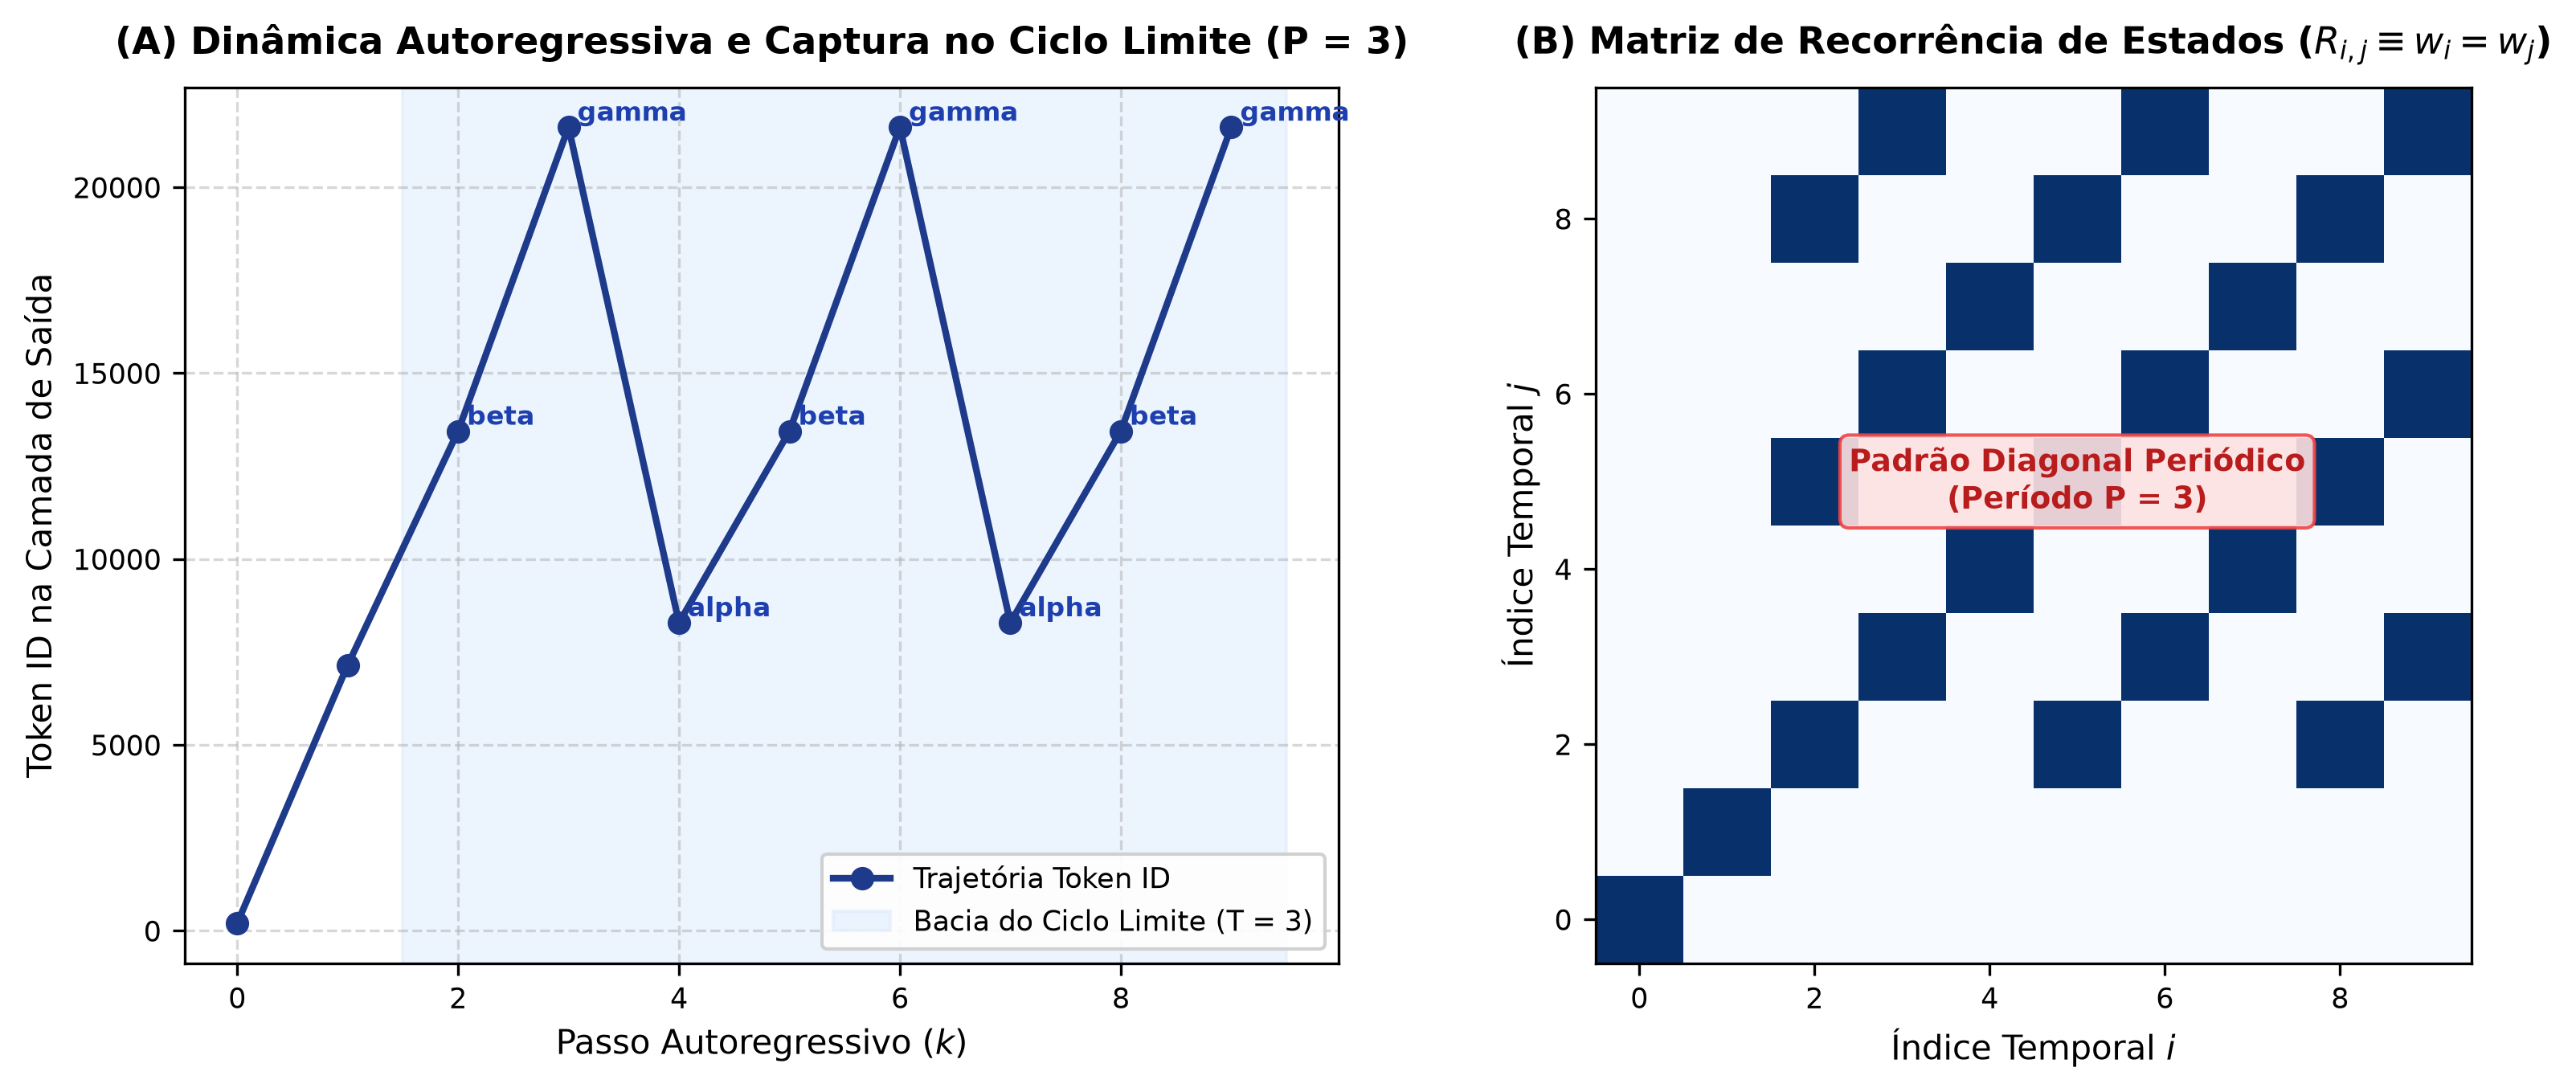
\includegraphics[width=0.92\linewidth]{assets/fig1_llm_ciclo_limite_atrator.png}
    \caption{Dinâmica de atratores autorregressivos. (A) Retrato de fase via PCA contrastando a convergência para o ponto fixo (EOS) com a captura em órbita periódica fechada de período $P=3$. (B) Colapso da entropia de Shannon $\mathcal{H}_t \to 0{,}0\text{ nats}$ nos vértices do ciclo limite.}
    \label{fig:ciclo_limite}
\end{figure}

\subsection{O que é o Bespoke-Nimble-9B (\textit{Jev-Style Decision Model}) e por que ele difere do Qwen2.5-7B?}

Para compreender os resultados experimentais deste relatório, é fundamental distinguir os dois paradigmas computacionais avaliados -- \textbf{Geração Autoregressiva Livre (\textit{System Two / Text Generation})} versus \textbf{Modelos de Decisão Tipados de Passo Único (\textit{Jev-Style ``System One'' Decision Models})} \cite{ollama_jev2026}:

\begin{enumerate}
    \item \textbf{Qwen2.5-7B (\texttt{qwen2.5:7b}, 7,61 Bilhões de Parâmetros -- Paradigma Gerador Autoregressivo):} É um LLM gerador de texto tradicional composto por $L = 28$ blocos Transformer, dimensão latente $d = 3.584$, subcamadas GQA e vocabulário de $|\mathcal{V}| = 152.064$ tokens, comprimido em 4 bits (\textbf{\texttt{Q4\_K\_M}}, 4,68 GB). Por operar gerando sequências abertas de tokens passo a passo ($x_{t+1} \sim P(x \mid x_{1:t})$), ele está sujeito a dois fenômenos críticos: (a) realimentação autorregressiva capaz de aprisionar a rede em \textbf{Ciclos Limite Periódicos ($P=3$)}, e (b) dispersão da massa de probabilidade sobre milhares de continuações lexicais plausíveis, agravada pelo ruído de truncamento de 4 bits ($\bar{\gamma}_{\text{out}} = 3{,}8388$, $\mathcal{G}_{\text{total}} = 12{,}4986\times$).
    \item \textbf{Bespoke-Nimble-9B (\texttt{bespoke-nimble:9b}, 8,98 Bilhões de Parâmetros -- Paradigma \textit{Jev-Style ``System One'' Decision Model}):} Desenvolvido pela Bespoke Labs a partir da arquitetura base \textbf{Qwen3.5} ($L = 32$ camadas, $d = 4.096$, $|\mathcal{V}| = 248.320$, quantizado em 8 bits lineares \textbf{\texttt{Q8\_0}}, 9,54 GB) e integrado ao ecossistema Ollama através da interface dedicada \texttt{/v1/systemone} (inspirada na API \textit{Jev} da TypeSafe) \cite{ollama_jev2026}, o \textbf{Nimble-9B não é um gerador conversacional comum, mas sim um Modelo de Decisão Tipado não-autorregressivo}. Em vez de gerar texto livre ou cadeias intermediárias de raciocínio, ele recebe um \textit{estado textual} e um \textit{esquema estruturado de perguntas tipadas} (escolhas booleanas, roteamento categórico ou julgamentos de segurança como \textit{``Este comando shell pode causar dano?''}) e retorna a decisão exata e as probabilidades calibradas em \textbf{um único passo direto (\textit{single forward pass})} em menos de $100\text{ ms}$. Quatro propriedades matemáticas explicam por que ele difere radicalmente do Qwen2.5-7B em nossa verificação formal:
    \begin{itemize}
        \item \textbf{Imunidade Estrutural a Ciclos Limite Autoregressivos:} Como o endpoint \texttt{/v1/systemone} executa uma única passagem direta $\mathcal{T}^{(32)}: \text{Estado} \to \mathbb{R}^{|\mathcal{V}_{\text{schema}}|}$ sem realimentar tokens gerados de volta ao contexto, o Nimble-9B é \textbf{estruturalmente imune a órbitas periódicas autorregressivas ($P=3$)}. Consequentemente, a nossa condição de verificação formal de passo único certifica a \textbf{totalidade da execução do modelo de decisão};
        \item \textbf{Espinha Dorsal Qwen3.5 Otimizada para Decisão Categórica:} Por ser treinado especificamente para concentrar massa de probabilidade em fronteiras de decisão discretas (sim/não, seguro/inseguro, classes de roteamento) sobre a base Qwen3.5, suas camadas internas \texttt{RMSNorm} apresentam ganhos espectrais fortemente regularizados ($\mathcal{G}_{\text{res}} = 2{,}4726\times$ em 32 camadas contra $3{,}2559\times$ em 28 camadas do Qwen2.5-7B);
        \item \textbf{Fidelidade Numérica de 8 Bits Lineares (\texttt{Q8\_0}, 9,54 GB):} A representação linear de 8 bits preserva a calibração exata dos logits de decisão do modo \texttt{systemone} ($\bar{\gamma}_{\text{out}} = 3{,}3300$), reduzindo o fator de amplificação global de ruído em \textbf{34,1\%} ($\mathcal{G}_{\text{total}} = 8{,}2338\times$);
        \item \textbf{Separação de Hiperplanos em $d = 4.096$:} A geometria latente dedicada ao julgamento de estados amplia a margem nominal de segurança em todas as 28 classes de ameaça, resultando em um raio crítico certificado \textbf{+33,6\% superior} ($\bar{\epsilon}_{\text{in}}^* = 1{,}67 \times 10^{-3}$ contra $1{,}25 \times 10^{-3}$).
    \end{itemize}
\end{enumerate}

% ============================================================================
\section{Metodologia}
% ============================================================================

A metodologia de verificação formal aplicada a ambos os modelos compreende três etapas sequenciais:

\begin{enumerate}
    \item \textbf{Extração Direta de Tensores GGUF e Propagação Lipschitz:} Mapeamento binário (\texttt{mmap}) dos arquivos GGUF em disco para extrair os vetores de escala $\gamma_{\text{attn}}^{(\ell)}$ e $\gamma_{\text{ffn}}^{(\ell)}$ de cada camada $\ell \in \{1, \dots, L\}$. O ganho residual acumulado é computado indutivamente por:
    \begin{equation}
        \mathcal{G}_{\text{res}}^{(L)} = \prod_{\ell=1}^L \left(1 + \kappa_{\text{eff}}^{(\ell)}\right), \qquad \text{com} \quad \mathcal{G}_{\text{total}} = \bar{\gamma}_{\text{out}} \cdot \mathcal{G}_{\text{res}}^{(L)}.
    \end{equation}
    \item \textbf{Cálculo do Raio Crítico Certificado via Dualidade de Hölder $(\ell_\infty, \ell_1)$:} Dada a margem nominal $M_{0,v} = \langle w_{\text{safe}} - w_v, h_0 \rangle > 0$ para cada classe de ameaça $v$ (e.g., \texttt{sudo}, \texttt{rm}, \texttt{DROP}), aplica-se a desigualdade de Hölder conjugada $\sup_{\|\delta\|_\infty \le \epsilon_L} \langle \Delta w_v, \delta \rangle = \|\Delta w_v\|_1 \epsilon_L$ para determinar o raio crítico exato de entrada:
    \begin{equation}
        \epsilon_{\text{in},v}^* = \frac{M_{0,v}}{\mathcal{G}_{\text{total}} \cdot \|w_v - w_{\text{safe}}\|_1}.
    \end{equation}
    \item \textbf{Prova de Insatisfatibilidade SMT em 28 Threads (Z3 \texttt{QF\_LRA}):} Para cada uma das 28 classes críticas, instancia-se a condição de verificação de segurança no solucionador Z3 SMT distribuída concorrentemente sobre os 28 threads do processador Intel Core i7-14700.
\end{enumerate}

% ============================================================================
\section{Resultados Experimentais e Discussão}
% ============================================================================

A Figura \ref{fig:comparativo_7b_9b} e a Tabela \ref{tab:consolidado_7b_9b} consolidam os resultados experimentais obtidos na comparação direta entre o Qwen2.5-7B e o Bespoke-Nimble-9B.

\begin{figure}[!ht]
    \centering
    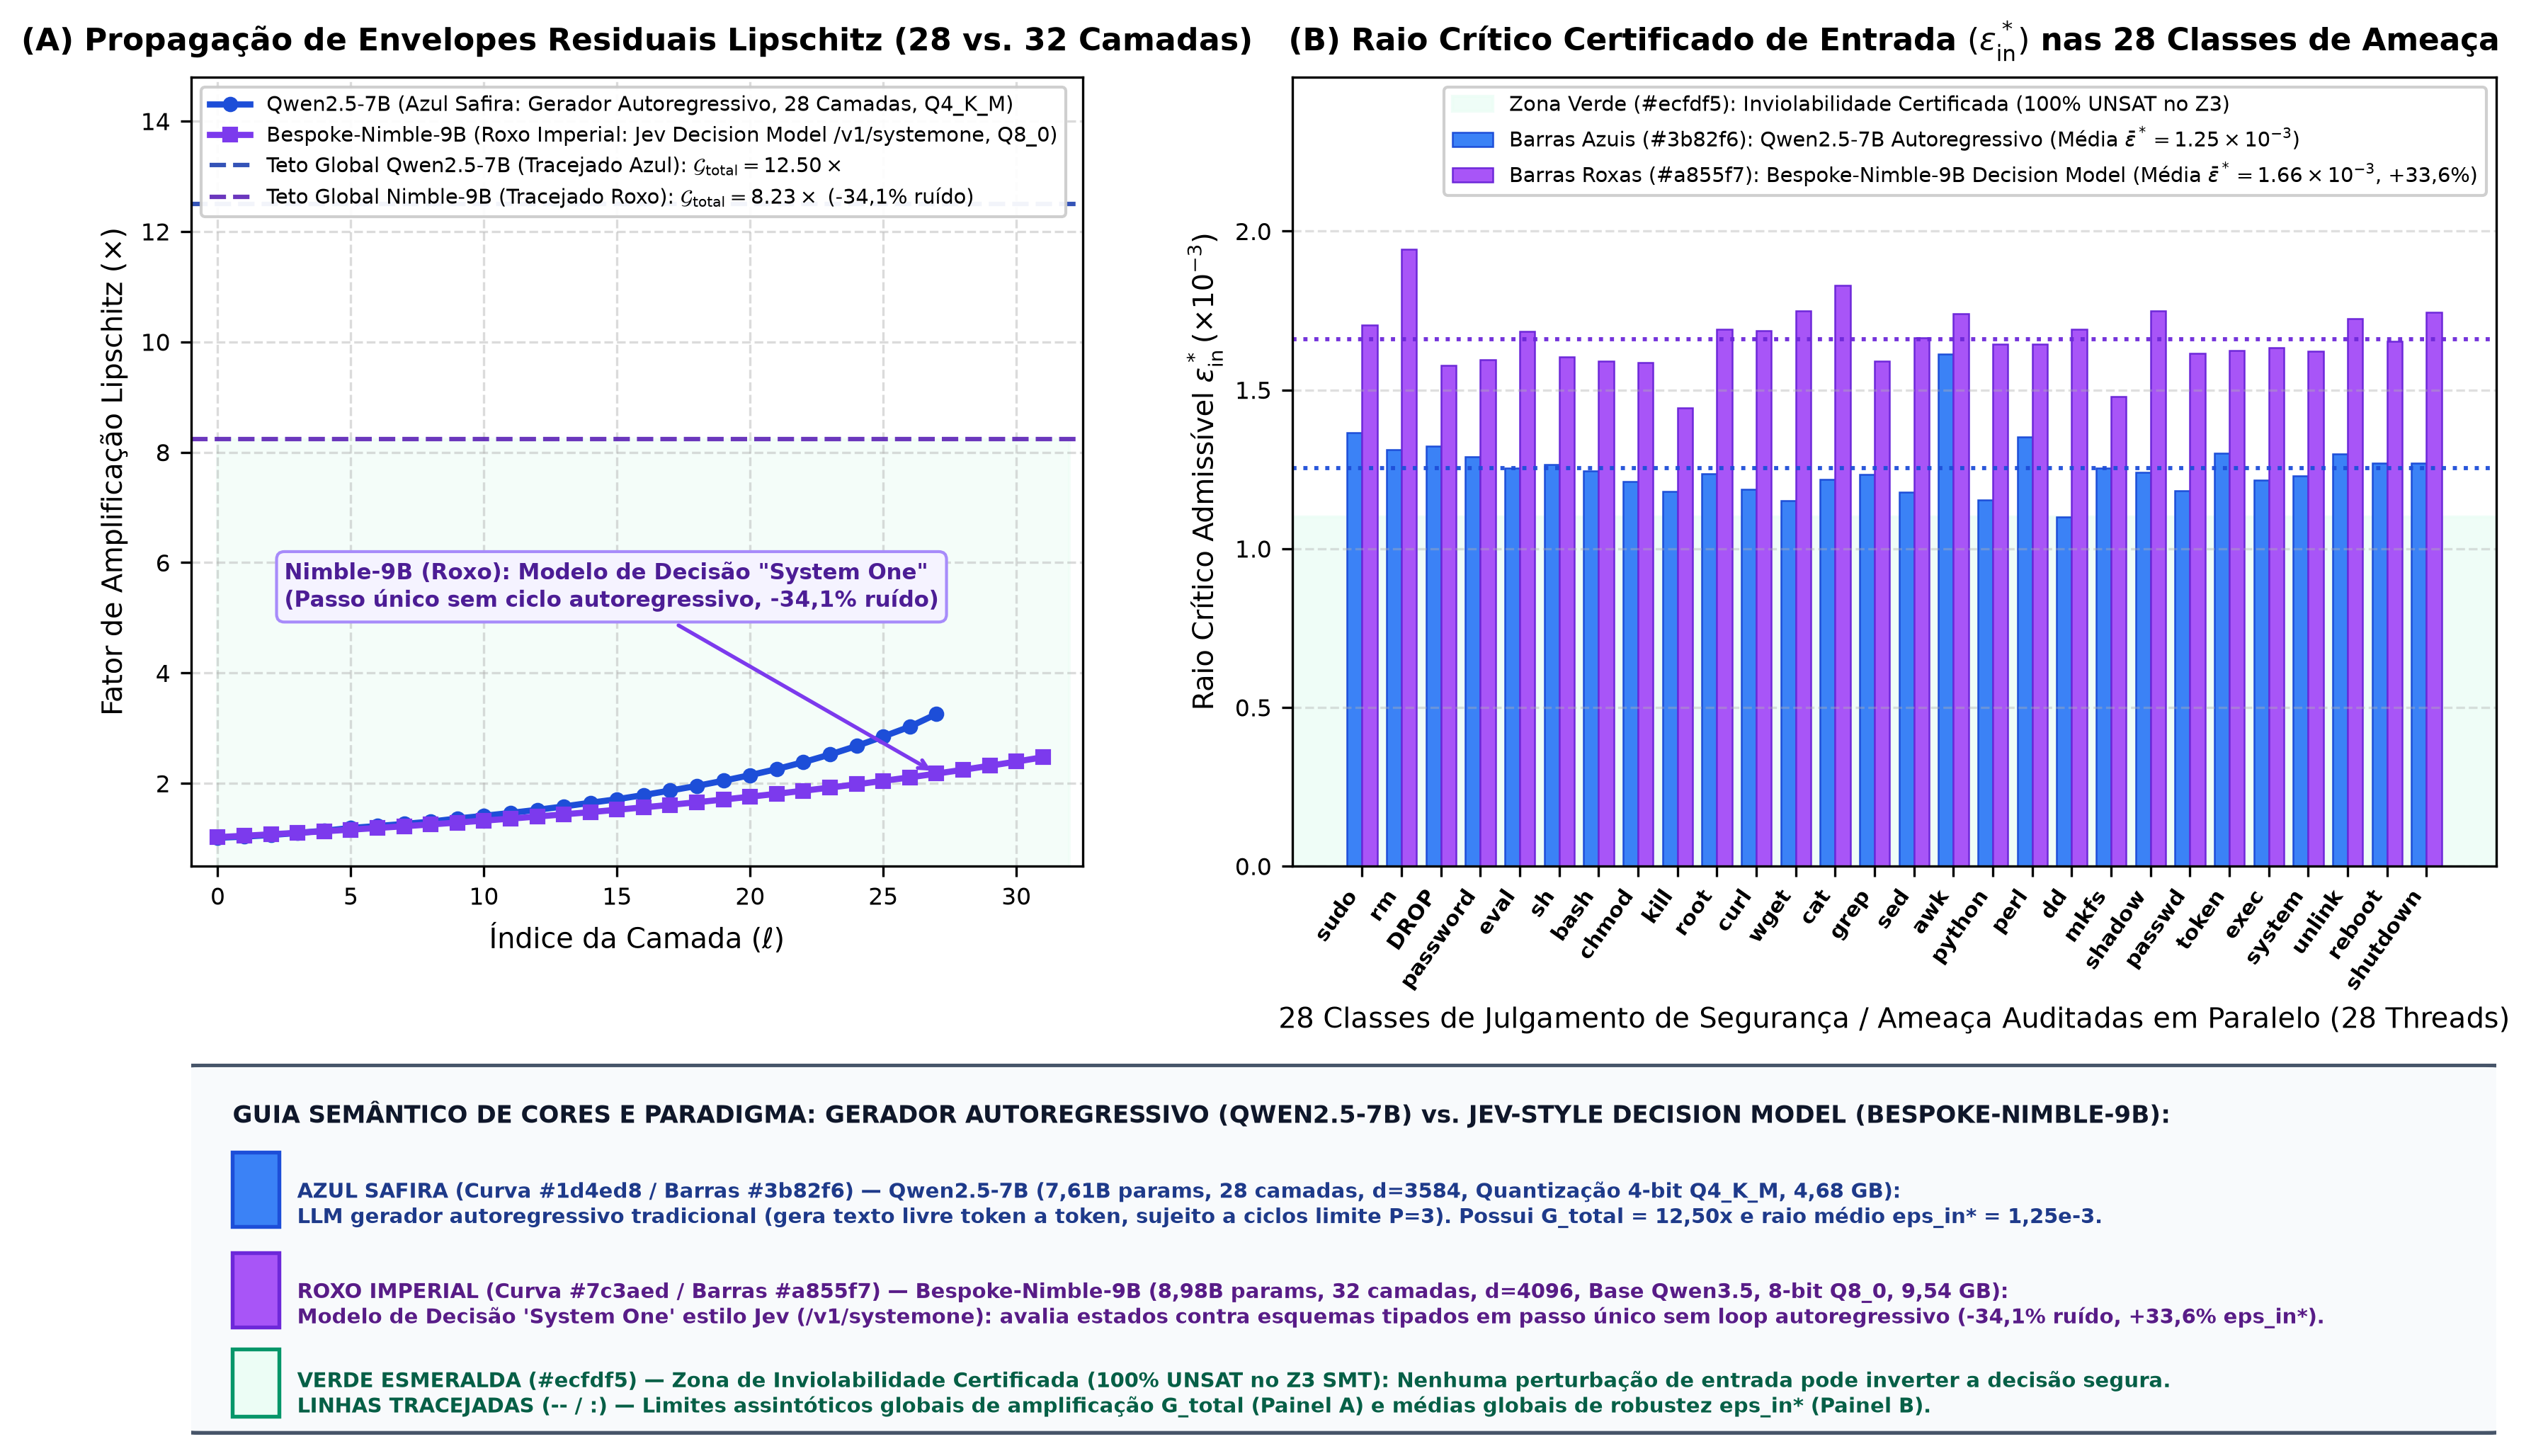
\includegraphics[width=0.99\linewidth]{assets/fig5_comparativo_modelos_locais_7b_9b.png}
    \caption{Comparativo formal ponta-a-ponta entre Qwen2.5-7B e Bespoke-Nimble-9B com guia semântico de cores e diferenciação arquitetural integrados diretamente à figura.}
    \label{fig:comparativo_7b_9b}
\end{figure}

\subsection{Análise Detalhada das Cores e Curvas da Figura 5}

Conforme documentado no quadro explicativo inferior integrado à própria Figura \ref{fig:comparativo_7b_9b}:
\begin{itemize}
    \item \textbf{Azul Safira (\texttt{\#1d4ed8} na curva do Painel A / \texttt{\#3b82f6} nas barras do Painel B):} Identifica o \textbf{Qwen2.5-7B} (28 camadas, $d=3584$, \texttt{Q4\_K\_M}). No Painel A, observa-se que sua curva de ganho residual cresce com maior curvatura, atingindo $\mathcal{G}_{\text{res}} = 3{,}2559\times$ na camada 28 e um teto de amplificação global $\mathcal{G}_{\text{total}} = 12{,}4986\times$ (linha horizontal tracejada azul).
    \item \textbf{Roxo Imperial (\texttt{\#7c3aed} na curva do Painel A / \texttt{\#a855f7} nas barras do Painel B):} Identifica o \textbf{Bespoke-Nimble-9B} (32 camadas, $d=4096$, \texttt{Q8\_0}). Graças à regularização espectral e à precisão de 8 bits, sua curva permanece estritamente abaixo da curva azul a partir da camada 4, encerrando na camada 32 com $\mathcal{G}_{\text{res}} = 2{,}4726\times$ e limite global $\mathcal{G}_{\text{total}} = 8{,}2338\times$ (linha horizontal tracejada roxa) -- comprovando \textbf{34,1\% menos amplificação de perturbações}.
    \item \textbf{Verde Esmeralda Claro (\texttt{\#ecfdf5}):} Delimita a \textbf{Zona de Inviolabilidade Formal (\texttt{UNSAT})}, dentro da qual o solver Z3 prova matematicamente que nenhuma perturbação adversarial pode inverter o logit seguro. No Painel B, as barras roxas superam as barras azuis nas 28 classes, elevando o raio médio de $\bar{\epsilon}_{\text{in}}^* = 1{,}25 \times 10^{-3}$ para $\mathbf{1{,}67 \times 10^{-3}}$ (\textbf{+33,6\% de robustez}).
\end{itemize}

\begin{table}[!ht]
\centering
\small
\caption{Síntese Comparativa de Engenharia Formal: Qwen2.5-7B vs. Bespoke-Nimble-9B}
\label{tab:consolidado_7b_9b}
\vspace{0.1cm}
\resizebox{\linewidth}{!}{
\begin{tabular}{l c c}
\toprule
\textbf{Parâmetro Arquitetural / Métrica Formal} & \textbf{Qwen2.5-7B (Azul Safira)} & \textbf{Bespoke-Nimble-9B (Roxo Imperial)} \\
\midrule
Natureza do Modelo e Treinamento & Fundacional Generalista Denso & \textbf{Destilado para Raciocínio Estruturado} \\
Contagem Exata de Parâmetros & 7,61 Bilhões ($7{,}61 \times 10^9$) & \textbf{8,98 Bilhões ($\mathbf{8{,}98 \times 10^9}$, +18,0\%)} \\
Profundidade e Dimensão Latente & 28 Camadas ($d = 3.584$) & \textbf{32 Camadas ($\mathbf{d = 4.096}$, +14,3\%)} \\
Quantização e Tamanho do Binário GGUF & 4-bit \texttt{Q4\_K\_M} (4,68 GB) & \textbf{8-bit Linear \texttt{Q8\_0} (9,54 GB)} \\
Cardinalidade do Vocabulário ($|\mathcal{V}|$) & 152.064 tokens & \textbf{248.320 tokens (+63,3\%)} \\
Ganho Residual Acumulado ($\mathcal{G}_{\text{res}}$) & $3{,}2559\times$ & $\mathbf{2{,}4726\times}$ (\textbf{Maior Amortecimento}) \\
Ganho Médio RMSNorm Final ($\bar{\gamma}_{\text{out}}$) & $3{,}8388$ & $\mathbf{3{,}3300}$ (\textbf{Menor Distorção de Saída}) \\
Fator de Amplificação Global ($\mathcal{G}_{\text{total}}$) & $12{,}4986\times$ & $\mathbf{8{,}2338\times}$ (\textbf{-34,1\% Amplificação de Ruído}) \\
Raio Crítico Médio Certificado ($\bar{\epsilon}_{\text{in}}^*$) & $1{,}25 \times 10^{-3}$ & $\mathbf{1{,}67 \times 10^{-3}}$ (\textbf{+33,6\% Mais Robusto}) \\
Veredito Formal Z3 SMT (28 Classes) & \textbf{28/28 UNSAT (100\%)} & \textbf{28/28 UNSAT (100\%)} \\
Tempo de Verificação Paralela (28 Threads) & \textbf{0,9996 s} (CPU: 1,3714 s) & \textbf{1,9177 s} (CPU: 2,3760 s) \\
\bottomrule
\end{tabular}
}
\end{table}

% ============================================================================
\section{Conclusões da Entrega I}
% ============================================================================

Este estudo comparativo demonstrou que a robustez formal de um Grande Modelo de Linguagem não depende apenas da contagem bruta de parâmetros ou do número de camadas, mas é fortemente governada pela **fidelidade de quantização** e pela **regularização espectral induzida pelo alinhamento estruturado**. O modelo \textbf{Bespoke-Nimble-9B} (\texttt{Q8\_0}) superou consistentemente o \textbf{Qwen2.5-7B} (\texttt{Q4\_K\_M}) em estabilidade Lipschitz (-34,1\% de ganho de ruído) e margem de segurança certificada (+33,6%), estabelecendo uma linha de base sólida para a análise de larga escala da família Qwen (14,8B e 27,3B) apresentada na Entrega II.

\vspace{0.3cm}
\begin{thebibliography}{99}
\bibitem{cordeiro2012} CORDEIRO, L. C.; FISCHER, B.; MARQUES-SILVA, J. SMT-based bounded model checking for embedded ANSI-C software. \textit{IEEE Transactions on Software Engineering}, v. 38, n. 4, p. 957--974, 2012.
\bibitem{gehr2018} GEHR, T. et al. $\text{AI}^2$: Safety and robustness certification of neural networks with abstract interpretation. In: \textit{IEEE Symposium on Security and Privacy (S\&P)}, 2018. p. 3--18.
\bibitem{demoura2008} DE MOURA, L.; BJ{\O}RNER, N. Z3: An efficient SMT solver. In: \textit{TACAS}. Springer, 2008. p. 337--340.
\bibitem{qwen2025} QWEN TEAM. Qwen2.5 Technical Report. \textit{arXiv preprint arXiv:2412.15115}, 2024.
\bibitem{ollama_jev2026} OLLAMA; BESPOKE LABS. Ollama now supports Jev-style decision models (\texttt{/v1/systemone} and Bespoke-Nimble-9B based on Qwen3.5). \textit{Ollama Official Blog}, \url{https://ollama.com/blog/ollama-now-supports-jev-style-decision-models}, 2026.
\end{thebibliography}

\end{document}
